%Document the algorithms we ported to SONIC, i.e., ParticleNet~\cite{Qu:2019gqs} + DeepTau~\cite{CMS:2022prd} + DeepMET. Include the algorithms and their implementations in CMSSW. Tables and PieChart about the latency breakdowns of these algorithms for Run-2 and Run-3. Discuss ragged batching? What about ECAL DRN? cite ECAL-specific note when released

%\textcolor{red}{Include IO sizes for these models. maybe also add them into Table~\ref{table:SONIC_Algos}}.

As mentioned in Section~\ref{sec:implementation}, one of the steps of CMS data processing is the creation of Mini-AOD files. These are designed to be relatively small and accessible, providing the high-level physics information needed for most analyses. They are derived from the AOD data format, reducing the size per event by a factor of 10.
Mini-AOD processing involves a wide variety of algorithms that propagate, skim, and reanalyze the AOD input objects. Figure~\ref{fig:algorithms} shows that the per-event latency is about 993\unit{ms} when processing simulated LHC Run 2  (proton-proton collisions at a center-of-mass energy of 13 TeV) \ttbar events on a 20-core Intel Haswell machine, when it is running five synchronized four-threaded jobs.

\begin{figure}[htp]
    \centering
    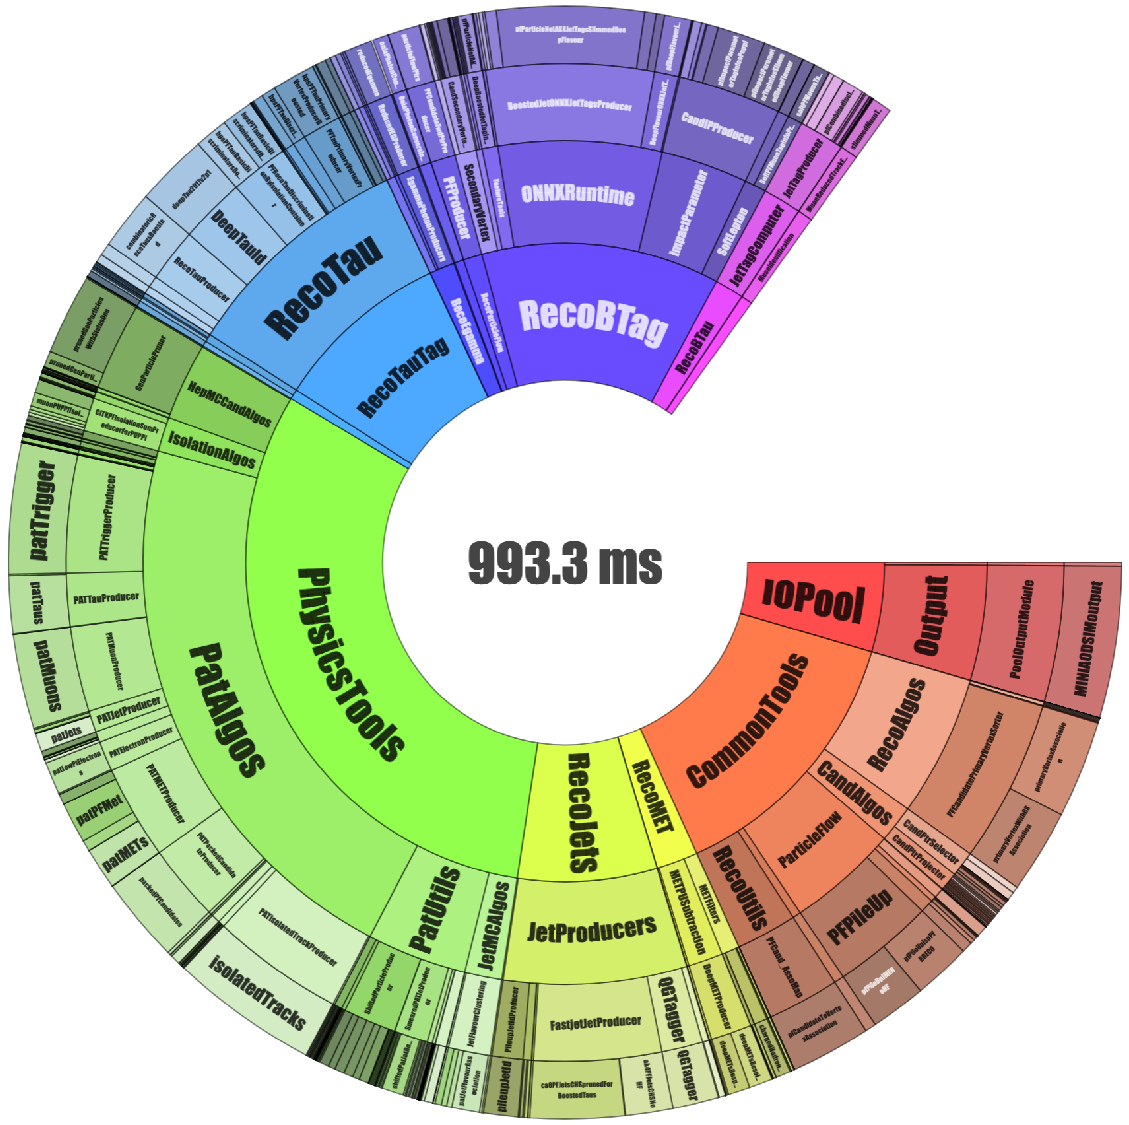
\includegraphics[width=0.50\textwidth]{plots/Step2_pieChart.pdf}
    \caption{Pie chart representing the per-event latency of various algorithms in a typical Mini-AOD processing for LHC Run 2 \ttbar events.}
    \label{fig:algorithms}
\end{figure}

\subsection{Algorithms}

There are three ML-based algorithms in the Mini-AOD workflow that are computing-intensive and relatively straightforward to execute in the SONIC paradigm:

\subsubsection{ParticleNet}
\label{sec:PN}

ParticleNet (PN)~\cite{Qu:2019gqs} is a graph neural network for jet tagging and regression that represents jets as ``particle clouds''. Here, ``tagging'' refers to identifying jets as arising from specific particles. PN was trained in \PYTORCH~\cite{pytorch}, which is a framework not currently supported in \CMSSW, and exported to the \ONNX format~\cite{onnx}, which \textit{is} supported in CMSSW for fast inference. However, it is important to note that with SONIC, it is possible to perform inference with PN in the following formats: \ONNX; \PYTORCH; and \PYTORCH with TensorRT (TRT)~\cite{tensorRT}, which optimizes model performance on NVIDIA devices.

There are four different trained versions of PN currently running in the Mini-AOD workflow for different purposes:
\begin{enumerate}
    \item tagging anti-\kt jets~\cite{Cacciari:2008gp}, clustered with the \FASTJET package~\cite{Cacciari:2011ma}, with a radius of 0.4 (AK4 jets),
    \item tagging anti-\kt jets with a radius of 0.8 (AK8 jets)~\cite{Sirunyan:2020lcu},
    \item mass-decorrelated tagging for AK8 jets~\cite{Sirunyan:2020lcu}, and
    \item mass regression for AK8 jets~\cite{CMS-DP-2021-017}.
\end{enumerate}
All PN variations can be hosted on Triton servers.

The inputs to PN are the kinematic and flavor properties of the particle constituents of each jet and the secondary vertices associated with the jet. The inputs are permutation invariant, and information for up to 100 particles and 10 vertices is used; if there are more than 100 particles in a jet, the 100 particles with the highest \pt are used. For the three tagging versions of PN, the outputs of each inference are category probabilities for a variety of pre-defined jet categories, such as the presence of a Higgs boson or the presence of a top quark. For the mass regression, the output is a single value: the predicted jet mass.

In Mini-AOD processing, inference is performed separately for each jet in a given event, so the number of PN inferences depends on the specific physics processes and can vary substantially from event to event. When running the standard \CMSSW version of PN, no inference batching is performed, so each inference is truly performed separately. In this context, each inference can have a variable number of inputs with no padding involved. When using SONIC for PN, it is easiest to batch all of the jets in an event into a single inference request, such that input particle and secondary vertex information for each jet in an event is sent to the server in a single request. In subsequent performance studies, a ``maximally-padded'' approach is taken, where every jet is padded to 100 particles and 10 vertices. This choice, and some alternatives are discussed in Section~\ref{sec:ragged}. In this configuration, a single 4-threaded job processing a Run 2 \ttbar event will generate about 140\unit{kB/s} of server input for AK4 jets and about 10\unit{kB/s} of server input for each of the AK8 jet versions of PN. At a processing rate of about 4 events per second, with about 16 AK4 jets per event, this corresponds about 2\unit{kB} of information per jet, which is consistent with the number of float inputs per jet.


\subsubsection{DeepMET}


The missing transverse momentum vector \ptvecmiss is typically computed as the negative vector sum of the transverse momenta of all the particles in an event, and its magnitude is denoted as \ptmiss~\cite{CMS:2019ctu}. DeepMET (DM)~\cite{DeepMET} is a \TENSORFLOW-based~\cite{tensorflow} deep neural network model that estimates the \ptvecmiss in an event. The vector $\ptvecmiss$ is associated with either the production of neutrinos or potential BSM particles that could propagate through the detector interacting only weakly. The inputs to DM are 11 features from each particle-flow candidate~\cite{CMS:2017yfk} in an event, with zero-padding up to 4\,500 candidates for a given event. This zero-padding is necessary for both the standard version of DM and for its SONIC-enabled implementation; similarly, in both cases, only one inference is made per event. DM outputs two values for each event: the \ptvecmiss components in the $x$ and $y$ directions. Because every event necessarily has the same number of inputs, dynamic batching is automatically available via SONIC, aiding inference efficiency in cases where many client jobs make concurrent requests within a certain time window (as shown in Fig.~\ref{fig:algorithms}, each client thread will make a request about once per second). A single 4-threaded job processing a Run 2 \ttbar event will generate about 1.3\unit{MB/s} of server input for DM.

\subsubsection{DeepTauID}

DeepTaudID (DT)~\cite{CMS:2022prd} is a \TENSORFLOW-based deep neural network model to identity hadronic decayed tau leptons from the jet collections. The inputs to the network include low-level particle features of electrons/photons, muons, and neutral hadrons, and high-level event features. The output is a three-dimensional tensor, representing the probability that the candidate is produced in different types of decay modes. In the implementation of direct inference in CMSSW, the network is split into three sub-models. The first two networks process the lower-level input information separately, and the third network combines the information from the first two models with the high-level information and outputs the discriminator values. In the SONIC implementation, we use a combined model with zero-padded inputs, so that dynamic batching can be used and GPUs can be utilized more efficiently. A single 4-threaded job processing a Run 2 \ttbar event will generate about 4.7\unit{MB/s} of server input for DT, making it the most demanding algorithm explored in this study in terms of server input.
    
    %\item ECAL DRN maybe?  Maybe put that as a separate bullet or just put that in a separate section entirely

\subsection{Latency}

The latency breakdown for the three algorithms highlighted above in a sample of Run 2 \ttbar events is presented in Table~\ref{table:SONIC_Algos}. The per-event average processing time is about 1 second; PN consumes about 6\% of this time, while DM and DT take about 1\% and 2\%, respectively. Thus, for this sample of events, the SONIC-ported algorithms account for about 10\% of the total latency. It is worth noting that this fraction is sample-dependent; for example, if a sample has fewer jets per event, PN will consume a smaller fraction of the per-event latency. However, thanks to the excellent performance of ML algorithms, more and more algorithms used in CMS data processing are being converted to ML versions. These will all benefit from the use of coprocessors, meaning that a higher fraction of latency will be able to be accelerated with SONIC easily in the future.

\begin{table}[ht!]
\begin{center}
\begin{tabular}{c r r r}
 Algorithm & \multicolumn{1}{c}{Time [ms]} & \multicolumn{1}{c}{Fraction [\%]} & \multicolumn{1}{c}{Input [MB]}\\ %[0.5ex] 
 \hline
 ParticleNet & 62.1 & 6.3 & 0.05 \\
 DeepMET & 13.2 & 1.3 & 0.33 \\
 DeepTauID & 21.1 & 2.1 & 1.18 \\
 \hline
 PN+DM+DT & 96.4 & 9.7 & 1.56 \\ 
 \hline
 Total & 993.3 & 100.0 & -- \\ 
\end{tabular}
\caption{The latency of the Mini-AOD processing illustrated in Fig.~\ref{fig:algorithms}, which does not use SONIC. The latency of the algorithms for which a SONIC version was created are stated explicitly. They consume about 10\% of the total per-event latency. This table also contains the expected server input for each model type created per event in Run 2 \ttbar events.}
\label{table:SONIC_Algos}
\end{center}
\end{table}


\subsection{Ragged batching}
\label{sec:ragged}

In the SONIC paradigm, it is generally easiest to make one inference request per event for each model hosted as-a-service. For some models, such as PN, this entails making inference requests with batch size greater than 1, involving multiple objects with potentially different numbers of inputs. This introduces a subtlety with respect to padding. Older versions of Triton did not allow for ``ragged batching'', in which inference requests for models with a variable number of inputs can be combined into a single batch even if each request has a different number of inputs. Because of this, two approaches can be taken.

In a maximally-padded approach, every object would be padded to the same input size. For example, in PN each jet can be padded to 100 particles and 10 vertices. In this scenario, all inference requests, including those for different events, will have the same number of inputs, making dynamic batching across events possible. This maximally-padded case will consume unnecessary bandwidth, as a significant fraction of the data transfer will be padding.

To get around this, one can implement a ``pseudo-ragged'' version of models, where objects in an event are padded up to the largest size of a single object in that event. For the PN example, this means that jets in an event would be padded up to the number of particles and vertices found in the largest jet in its event. This reduces wasted bandwidth for a given request---for the Run 2 \ttbar sample explored here, the input bandwidth is reduced by about a factor of 2 overall. In this case, Triton will batch together jets from the same event, and if by some coincidence, two separate inference requests were made for events with the same maximal jet size, then dynamic batching between the inferences would be possible. However, that is rare, so in practice pseudo-ragged PN does not take advantage of dynamic batching.

In the large-scale Mini-AOD production tests described below, the benefits of dynamic batching make the maximally-padded scenario favorable in terms of latency reduction, as many client jobs will be making requests concurrently, and batching is beneficial to inference efficiency. In scenarios where only one or a few client jobs are running at once for a given server, then the pseudo-ragged version provides superior throughput. Recent releases of Triton started supporting ragged batching, which is a feature under study and benchmarks.% \textcolor{red}{Mention different versions of PN for different clients? Include results on this: performances with different types of batching? From Patrick: I now mention the different formats of PN in 4.1.1, and the performance comparison is shown in Figure 5}